\documentclass[10pt,a4paper]{article}
\usepackage[utf8]{inputenc}
\usepackage[T1]{fontenc}
\usepackage{lmodern}
\usepackage[french]{babel}
\usepackage[margin=1.7cm,top=1.4cm,bottom=1.3cm]{geometry}
\usepackage{graphicx,booktabs,hyperref,microtype}
\usepackage{titlesec}
\pagestyle{empty}
\setlength{\parindent}{0pt}\setlength{\parskip}{3pt}
\titleformat{\section}{\large\bfseries}{}{0em}{}
\titlespacing*{\section}{0pt}{6pt}{2pt}
\begin{document}
{\LARGE\bfseries Discriminateur à fraction constante numérique : étude du temps de montée et de la résolution temporelle}\\[2pt]
{\small Douaa Guermassi --- étude préliminaire, simulation Python et implémentation Verilog vérifiée (code : github.com/douaa-g)}

\section{Objectif}
Dans une ligne à temps de vol, la résolution temporelle dépend de la façon dont on date l'instant d'arrivée d'une impulsion numérisée. Un seuil fixe donne un décalage qui dépend de l'amplitude (\emph{time walk}) ; un discriminateur à fraction constante (CFD) date l'impulsion à une fraction fixe de son amplitude et supprime ce décalage. J'ai étudié ce principe sur des impulsions simulées : j'ai comparé seuil fixe et CFD numérique, puis j'ai vérifié une implémentation en virgule fixe en Verilog contre mon modèle Python. Il s'agit d'une étude du \emph{principe}, pas d'une analyse d'un module réel.

\section{Méthode}
\textbf{Impulsions.} Forme bi-exponentielle (montée 2~ns, descente 20~ns, valeurs illustratives), amplitudes uniformes entre 0,3 et 1 de l'amplitude maximale, bruit blanc gaussien (SNR = amplitude max / bruit rms), phase d'arrivée aléatoire à l'intérieur de l'échantillon, 4\,000 événements par point.
\textbf{Seuil fixe :} premier franchissement du seuil, interpolation linéaire. \textbf{CFD :} $y[n]=f\,x[n]-x[n-d]$, passage par zéro après armement (seuil $6\sigma$), interpolation linéaire ; $f=K/8$.
\textbf{Mesure :} écart-type de $t_{\text{estimé}}-t_{\text{vrai}}$ (décalage constant retiré), en ps, par voie. Les paramètres optimaux (seuil, $f$, $d$) sont choisis sur un jeu d'événements puis évalués sur un jeu indépendant. La résolution sur une différence de temps entre deux voies identiques est $\sqrt{2}$ fois plus grande.

\begin{center}
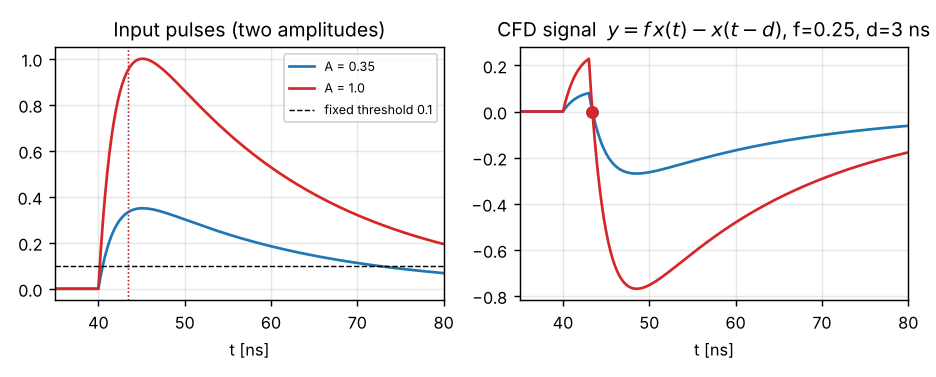
\includegraphics[width=0.78\linewidth]{figures/fig0_principle.png}
\end{center}

\section{Résultats}
\begin{minipage}[t]{0.49\linewidth}\centering
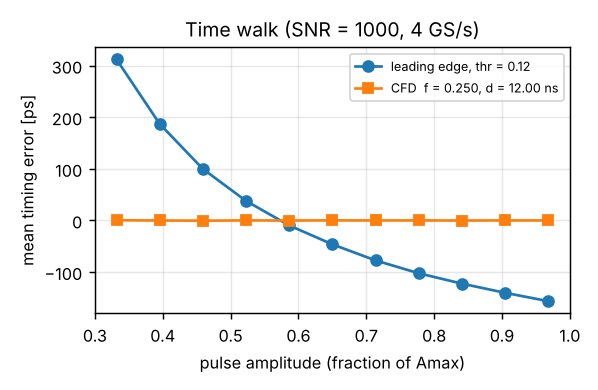
\includegraphics[width=\linewidth]{figures/fig1_walk.png}
\end{minipage}\hfill
\begin{minipage}[t]{0.49\linewidth}\centering
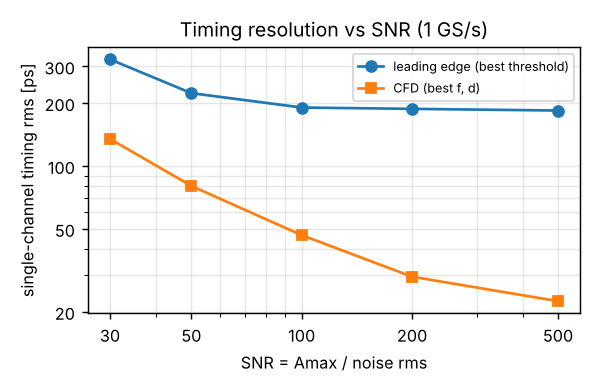
\includegraphics[width=\linewidth]{figures/fig2_snr.png}
\end{minipage}

\begin{minipage}[t]{0.49\linewidth}\centering
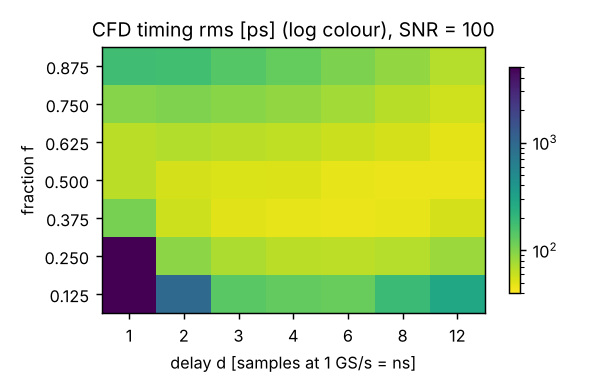
\includegraphics[width=\linewidth]{figures/fig3_heatmap.png}
\end{minipage}\hfill
\begin{minipage}[t]{0.49\linewidth}\centering
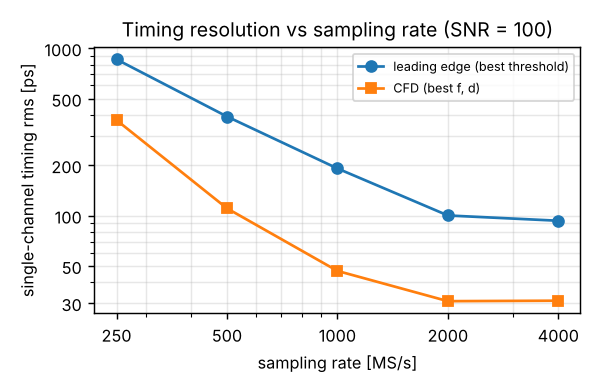
\includegraphics[width=\linewidth]{figures/fig4_fs.png}
\end{minipage}

\vspace{2pt}
\begin{itemize}\setlength{\itemsep}{1pt}
\item \textbf{Time walk :} sur la gamme d'amplitudes simulée, un seuil fixe donne un décalage de 469~ps crête à crête ; le CFD le ramène à moins de 1~ps (impulsions de même forme).
\item \textbf{Résolution :} à 1~GS/s et SNR = 100, 47~ps pour le meilleur CFD ($f=3/8$, $d=6$~ns) contre 194~ps pour le meilleur seuil fixe. L'écart se maintient pour tous les SNR testés (30 à 500) et toutes les cadences (250~MS/s à 4~GS/s).
\item \textbf{Réglage :} le résultat dépend peu de $(f,d)$ dans une large zone ($f$ de 3/8 à 5/8, $d\ge 3$~ns) ; les petits $f$ et petits $d$ sont à éviter (bruit).
\item \textbf{Cadence d'échantillonnage :} en dessous de 1~GS/s, la résolution se dégrade (372~ps à 250~MS/s), sans doute parce que le pas d'échantillonnage devient comparable au temps de montée et que l'interpolation linéaire est grossière ; au-delà de 2~GS/s, le gain sature.
\end{itemize}

\section{Implémentation Verilog et vérification}
Le CFD est décrit en Verilog (\texttt{rtl/cfd.v}) : échantillons signés sur 12 bits, $y=(K\,x\gg 3)-x[n-d]$, armement par seuil, détection du passage par zéro, verrouillage jusqu'à ce que le signal reste sous le seuil pendant 16 échantillons (sans ce dispositif, le bruit sur la queue de l'impulsion redéclenche l'unité : j'ai constaté 738 déclenchements pour 400 événements avant correction). Le module renvoie l'indice $n$ et $y[n-1]$, $y[n]$ ; l'interpolation sous-échantillon est faite en aval.
Un banc de test à fichiers (\texttt{tb/tb\_cfd.v}, Icarus Verilog) lit un flux de 400 impulsions quantifiées sur 12 bits et écrit les sorties ; un script Python les compare à un modèle en virgule fixe, bit à bit.

\begin{center}\small
\begin{tabular}{lc}\toprule
Vérification (400 événements, 1~GS/s, SNR = 100) & Résultat \\ \midrule
Sorties RTL = modèle Python en virgule fixe (bit à bit) & identiques (401 sorties) \\
Événements avec exactement un déclenchement & 399 / 400 \\
Résolution, CFD flottant non quantifié & 47,6~ps \\
Résolution, CFD flottant quantifié 12 bits & 47,6~ps \\
Résolution, sortie RTL en virgule fixe & 47,8~ps \\ \bottomrule
\end{tabular}
\end{center}

\section{Limites et suite}
Impulsions simulées de forme identique, bruit blanc seul, interpolation linéaire, cadence et forme d'impulsion illustratives : un détecteur réel présente une dispersion de temps de montée qui laisse un \emph{walk} résiduel, et le réglage optimal ($f$, $d$) dépend de la forme réelle. Prochaines étapes : tester sur des signaux numérisés réels, ajouter le bruit de gigue de l'horloge d'échantillonnage, comparer à une interpolation d'ordre supérieur, et ajouter un diviseur matériel pour l'interpolation.
\end{document}
